\documentclass{scrartcl}
    \usepackage{scrlayer-scrpage}
    \usepackage[czech]{babel}
    \usepackage{amsmath}
    \usepackage{graphicx}
    
    \cohead[Kombinatorika a grafy 2]
            {Kombinatorika a grafy 2}
    \lohead[Úkol č. 1]
            {Úkol č. 1}
    \rohead[Václav Luňák (Vašek)]
            {Václav Luňák (Vašek)}
    \pagestyle{plain.scrheadings}
    
    \graphicspath{ {./ukol1_imgs/} }

    \begin{document}
    \section{}
        Uvažme následující graf:
        \begin{center}
            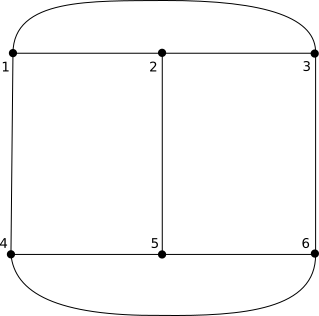
\includegraphics[height=5cm]{Graph1}
        \end{center}

        Tento graf je třísouvislý a nemá mosty. Dále uvažme hrany $(1,2)$ a $(5,6)$. Bude-li nějaké párování obsahovat obě tyto hrany, vrcholy 3 a 4 nelze nijak spárovat, tudíž žádné párování obsahující obě tyto hrany nemůže být perfektní.

    \section{}
        Mějme následující graf:
        \begin{center}
            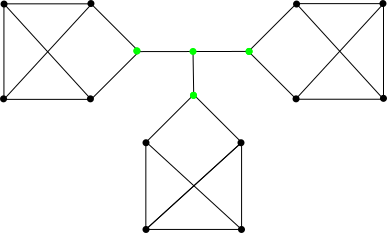
\includegraphics[height=5cm]{Graph2}
        \end{center}

        Tento graf je 3-regulární, ovšem pouze 1-souvislý (mezi zelenými vrcholy jsou mosty). Budeme hledat perfektní párování tohoto grafu. Kdybychom v jednom domečku spárovali černý vrchol se zeleným, zbydou v tomto domečku jen tři černé vrcholy, které již nelze všechny spárovat. V perfektním párování tedy musí být spárovány všechny černé vrcholy mezi sebou. \\

        Tím nám ovšem zbydou čtyři zelené vrcholy, které nelze žádným způsobem všechny spárovat. Tento graf tedy nemá perfektní párování.
    
    \section{}
        Párování grafu $K_{n,n}$ je ekvivalentní permutaci $n$ prvků (mezi $u_i$ a $w_j$ vede hrana právě tehdy, když $\pi(i) = j$). Počet těchto párování je tedy roven $n!$. Když z tohoto grafu odebereme jednu hranu, znemožníme právě párování používající tuto hranu. Tato párování jsou ekvivalentní permutacím s jedním konkrétním pevným bodem a je jich tedy $(n-1)!$ Počet párování výsledného grafu tedy vychází na $n! - (n-1)! = (n-1)! \cdot (n-1)$.
    
    \section{}
        Dokážeme indukcí. \\
        \begin{itemize}
            \item Strom s jedním vrcholem nemá žádné perfektní párování. Strom se dvěma vrcholy má právě jedno.
            \item Mějme strom $T$ o $n$ vrcholech ($n > 2$). Tento strom má nejméně dva listy. Vezmeme libovolný list stromu. Aby párování bylo perfektní, z tohoto listu musí vést párovací hrana. Vytvoříme strom $T'$ tak, že odebereme oba vrcholy této hrany z $T$. Tato operace nám nemůže porušit párování $T$, neboť oba odebrané vrcholy již byly spárovány. Zároveň je $T'$ les, jehož komponenty mají méně než $n$ vrcholů. Z indukčního předpokladu tedy existuje nejvýše jedno perfektní párování $T'$ (respektive všech jeho komponent). Zpětným přidáním vrcholů pak získáme nejvýše jedno perfektní párování $T$. (Jednoznačnost párování komponent $T'$ implikuje jednoznačnost párování $T$, protože komponenty $T'$ musí být v $T$ spojeny pouze nepárovacími hranami).
        \end{itemize}

    \section{}
        Graf $G_{n,a,b}$ je bipartitní graf. První partitu tvoří množina $M = \{ X :\vert X \vert = a\}$. Druhá partita je pak tvořena množinou $N = \{ X : \vert X \vert = b \}$. Toto dokážeme snadno z faktu, že množina nemůže být podmnožinou množiny stejné velikosti.\\

        Zároveň z definice vrcholů máme $\vert M \vert = \binom{n}{a}$ a $\vert N \vert = \binom{n}{b}$. Protože se jedná o bipartitní graf, velikost největšího párování může být rovna nejvýše velikosti menší z partit.\\

        Z každého vrcholu $N$ vede $\binom{b}{a}$ hran do vrcholů $M$. Tyto hrany totiž odpovídají všem podmnožinám velikosti $a$ z množiny velikosti $b$. Pokud $\vert N \vert \leq \vert M \vert$, vrcholy v $M$ mají stupně stejné nebo menší než $\binom{b}{a}$. Z libovolné množiny $J \subseteq N$ pak vede $\vert J \vert \cdot \binom{b}{a}$ hran. Z nižších stupňů vrcholů v $M$ ovšem dostáváme $\vert N(J) \vert \geq \frac{\binom{b}{a} \cdot \vert J \vert}{\binom{b}{a}}$, tudíž je splněna Hallova podmínka a $G_{n,a,b}$ má SRR. Pro $\vert N \vert \geq \vert M \vert$ je argument stejný, pouze vyměníme partity.\\

        $G_{n,a,b}$ tedy má SRR a velikost jeho největšího párování je rovna $\text{min}\{\binom{n}{b},\binom{n}{a}\}$
        
    \section{}
        Mějme dvě maximální párování, $X$ a $Y$. Jelikož $X$ je párování, musí platit, že každá hrana z $Y \backslash X$ sousedí nejvýše se dvěma hranami z $X \backslash Y$. V opačném případě bychom měli dvě hrany $X$ končící ve stejném bodě.\\
        
        Zároveň víme, že každá hrana z $X \backslash Y$ sousedí s alespoň jednou hranou z $Y \backslash X$. Kdyby to pro nějakou hranu neplatilo, dala by se přidat do $Y$, což je spor s jeho maximalitou.\\

        Z předchozích dvou pozorování tedy dostáváme, že $\vert X \backslash Y \vert \leq 2 \cdot \vert Y \backslash X \vert$. Dále pak úpravami:

        \begin{align*}
            \vert X \vert = \vert X \cap Y \vert + \vert X \backslash Y \vert \leq \vert X \cap Y \vert + 2 \cdot \vert Y \backslash X \vert \leq 2 \cdot \vert Y \cap X \vert + 2 \cdot \vert Y \backslash X \vert = 2 \cdot \vert Y \vert
        \end{align*}

        Z čehož nám vyplývá, že $\vert X \vert \leq 2 \cdot \vert Y \vert$ pro libovolná dvě maximální párování. Pokud za $X$ dosadíme nějaké největší párování grafu $G$, pak pro libovolné $Y$ maximální párování tohoto grafu dostáváme $\frac{ \mu (G)}{2} \leq \vert Y \vert$.
    \end{document}   